\section{Design and implementation details}

{\bf Here you describe a more detailed view of the various parts of the architecture describing how the robot controller or game was designed.}


\subsection{Skiller multiplayer framework}
Due to the desire of developing a fully functional multiplayer game, the \emph{Skiller multiplayer framework} \cite{skiller} has been used. This is a third party COTS software, and its usage has sped up the development process. Registration was needed in order to gain access to the Skiller SDK. When the registration was done, a new game could be created, and an application ID, an application key, and an application secret was supplied. These are used in the code to identify the specific application. \\

This framework supplies a server solution for turn based games, and it has been implemented in the network class. When playing a network game, the GameController class tells the Game model to  network class sends event messages to the server, and the server delivers it to the opponent.

\subsection{Activities}
Figure \ref{fig:activities} shows an overview of the application's different activities, and how the user interactions can change them. \\

\begin{figure}[H]
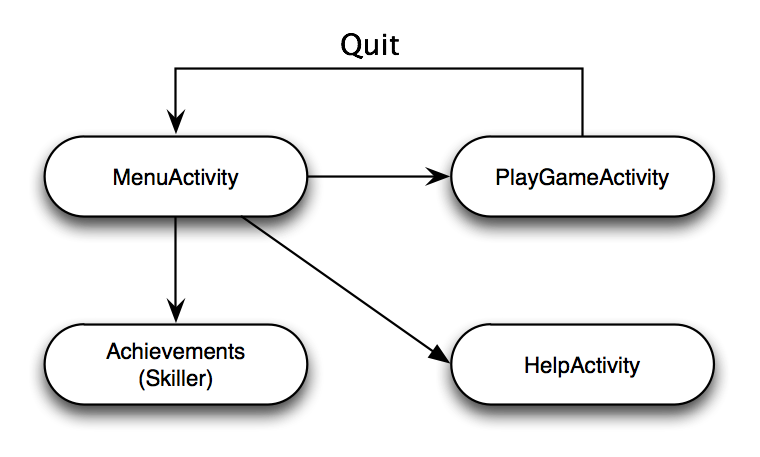
\includegraphics[width=1\textwidth]{Images/activities}
\caption{Application activities}
\label{fig:activities}
\end{figure}

The MenuActivity shows a menu consisting of five items, allowing the user to create or join a multiplayer game, start a local game, check achievements, or check the game rules. The PlayGameActivity is responsible for creating or joining multiplayer games, and starting local games. The HelpActivity is responsible for showing the game rules. The achievement screen is supplied by \emph{Skiller}.\\

Screencaps of the different activities, and the achievement screen, are shown in section \ref{section:playing}.
%\ref{section:label}

\subsection{MVC}
BoardView -> GameController -> Game model -> BoardView og Network (if(!hotseat))






